% !TeX root = ../main.tex

\chapter{个人贡献}

在此次大作业中,我负责最终汇报的 \textsc{Beamer} 幻灯片的编写与对算法 (\ref{Algorithm:RMFA}) 和 算法 (\ref{Algorithm:DFAS}) 性能对比分析。在使用由组内其他成员编写的测试脚本对两种算法进行对比实验后,可以得到多组数据。对这些数据求平均值便可以得到最终的性能对比分析数据,再使用 Python 绘图库即可绘制出具体的性能对比图。

\paragraph{\textsc{Beamer} 编写}

在编写 \textsc{Beamer} 幻灯片时,我们使用了在线 \LaTeX 编辑网站 \href{https://www.overleaf.com/}{Overleaf} 进行 \textsc{Beamer} 幻灯片的撰写,如图 (\ref{Overleaf}) 所示。
\begin{figure}[htb]
    \centering
    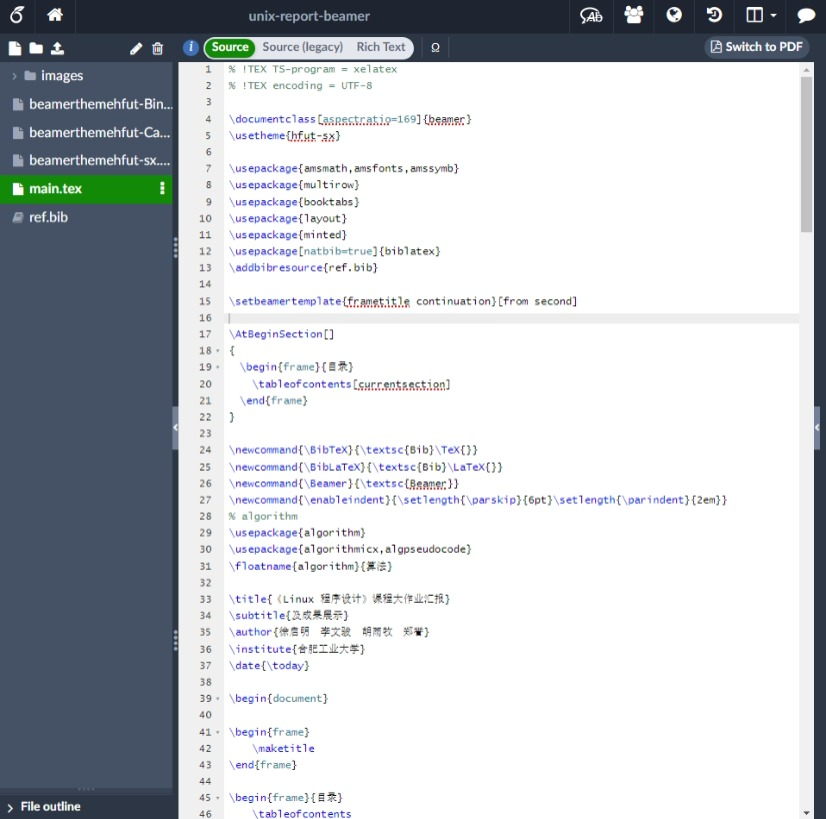
\includegraphics[width=0.45\textwidth]{figures/Overleaf.jpeg}
    \qquad
    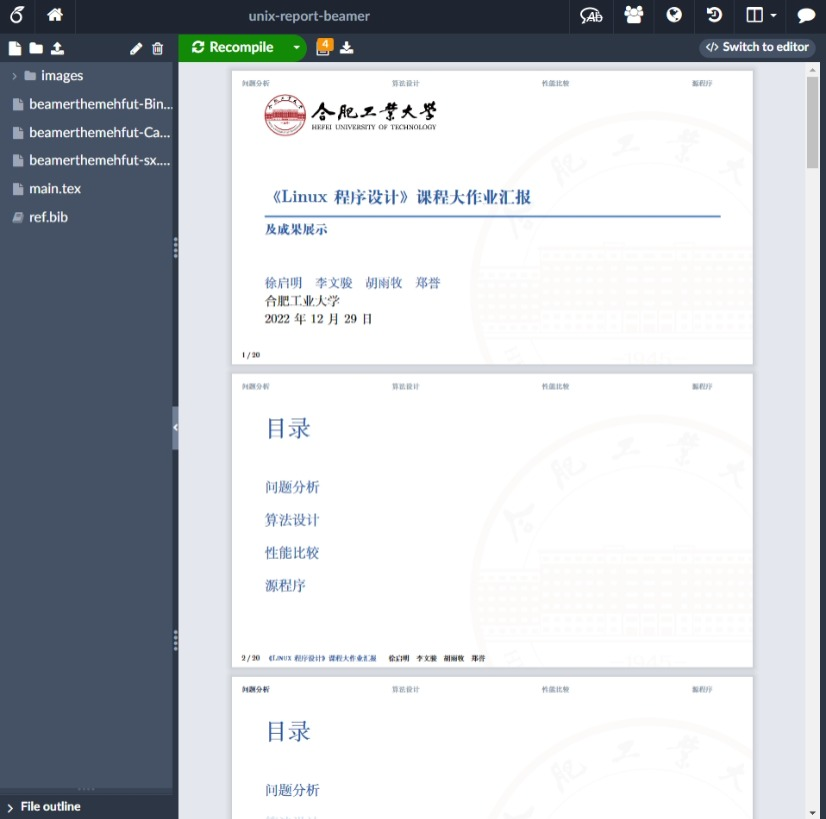
\includegraphics[width=0.45\textwidth]{figures/Beamer.jpeg}
    \caption{在线 \LaTeX 编辑网站 \href{https://www.overleaf.com/}{Overleaf}(左) 和我们最终的 \textsc{Beamer} 汇报成果(右)}
    \label{Overleaf}
\end{figure}

我们已经将 \textsc{Beamer} 报告的文档源代码上传至 GitHub 仓库:\href{https://github.com/xqm32/unix-report-latex}{https://github.com/xqm32/unix-report-latex}。

\paragraph{性能对比分析}

在进行性能对比实验时,我们对问题 (\ref{problem}) 中各个变量 $a,b,c,d$ 呈如下分布:
\begin{align}
    a & =|randn(1)|\nonumber  \\
    d & =randn(1)\nonumber    \\
    b & =randn(m, 1)\nonumber \\
    c & =randn(m, 1)\nonumber
\end{align}

记录 $m=10^2,10^3,10^4,10^5,10^6$ 时所消耗的时间,便可以绘制性能对比图像。

如图 (\ref{Draw}) 所示,我们使用 Python 语言的 matplotlib 绘图库进行性能对比分析的图像绘制。我们以 $log(m)$ 作为 $x$ 轴的,通过绘制不同的 $m$ 值下两个算法求解所消耗的时间曲线进行对两种算法的性能分析。
\begin{figure}[htb]
    \centering
    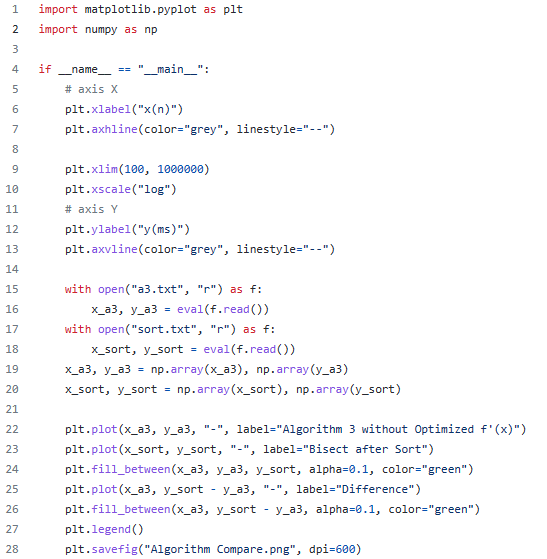
\includegraphics[width=0.5\textwidth]{figures/py@draw.png}
    \caption{绘图程序源代码}
    \label{Draw}
\end{figure}

通过使用图 (\ref{Draw}) 所示程序,我们可以得出如图 (\ref{Compare}) 所示的性能对比图。图中的橙色线为算法 (\ref{Algorithm:DFAS}) 的所用时间,蓝色线为算法 (\ref{Algorithm:RMFA}) 的所用时间,绿色线为两算法所耗时间的差值。不难看出,算法 (\ref{Algorithm:RMFA}) 相较于算法 (\ref{Algorithm:DFAS}) 在 $10^6$ 数量级的数据下快了将近 $\frac{1}{5}$。这也与我们在算法设计一节中所说明的算法时间复杂度相近。
\begin{figure}[htb]
    \centering
    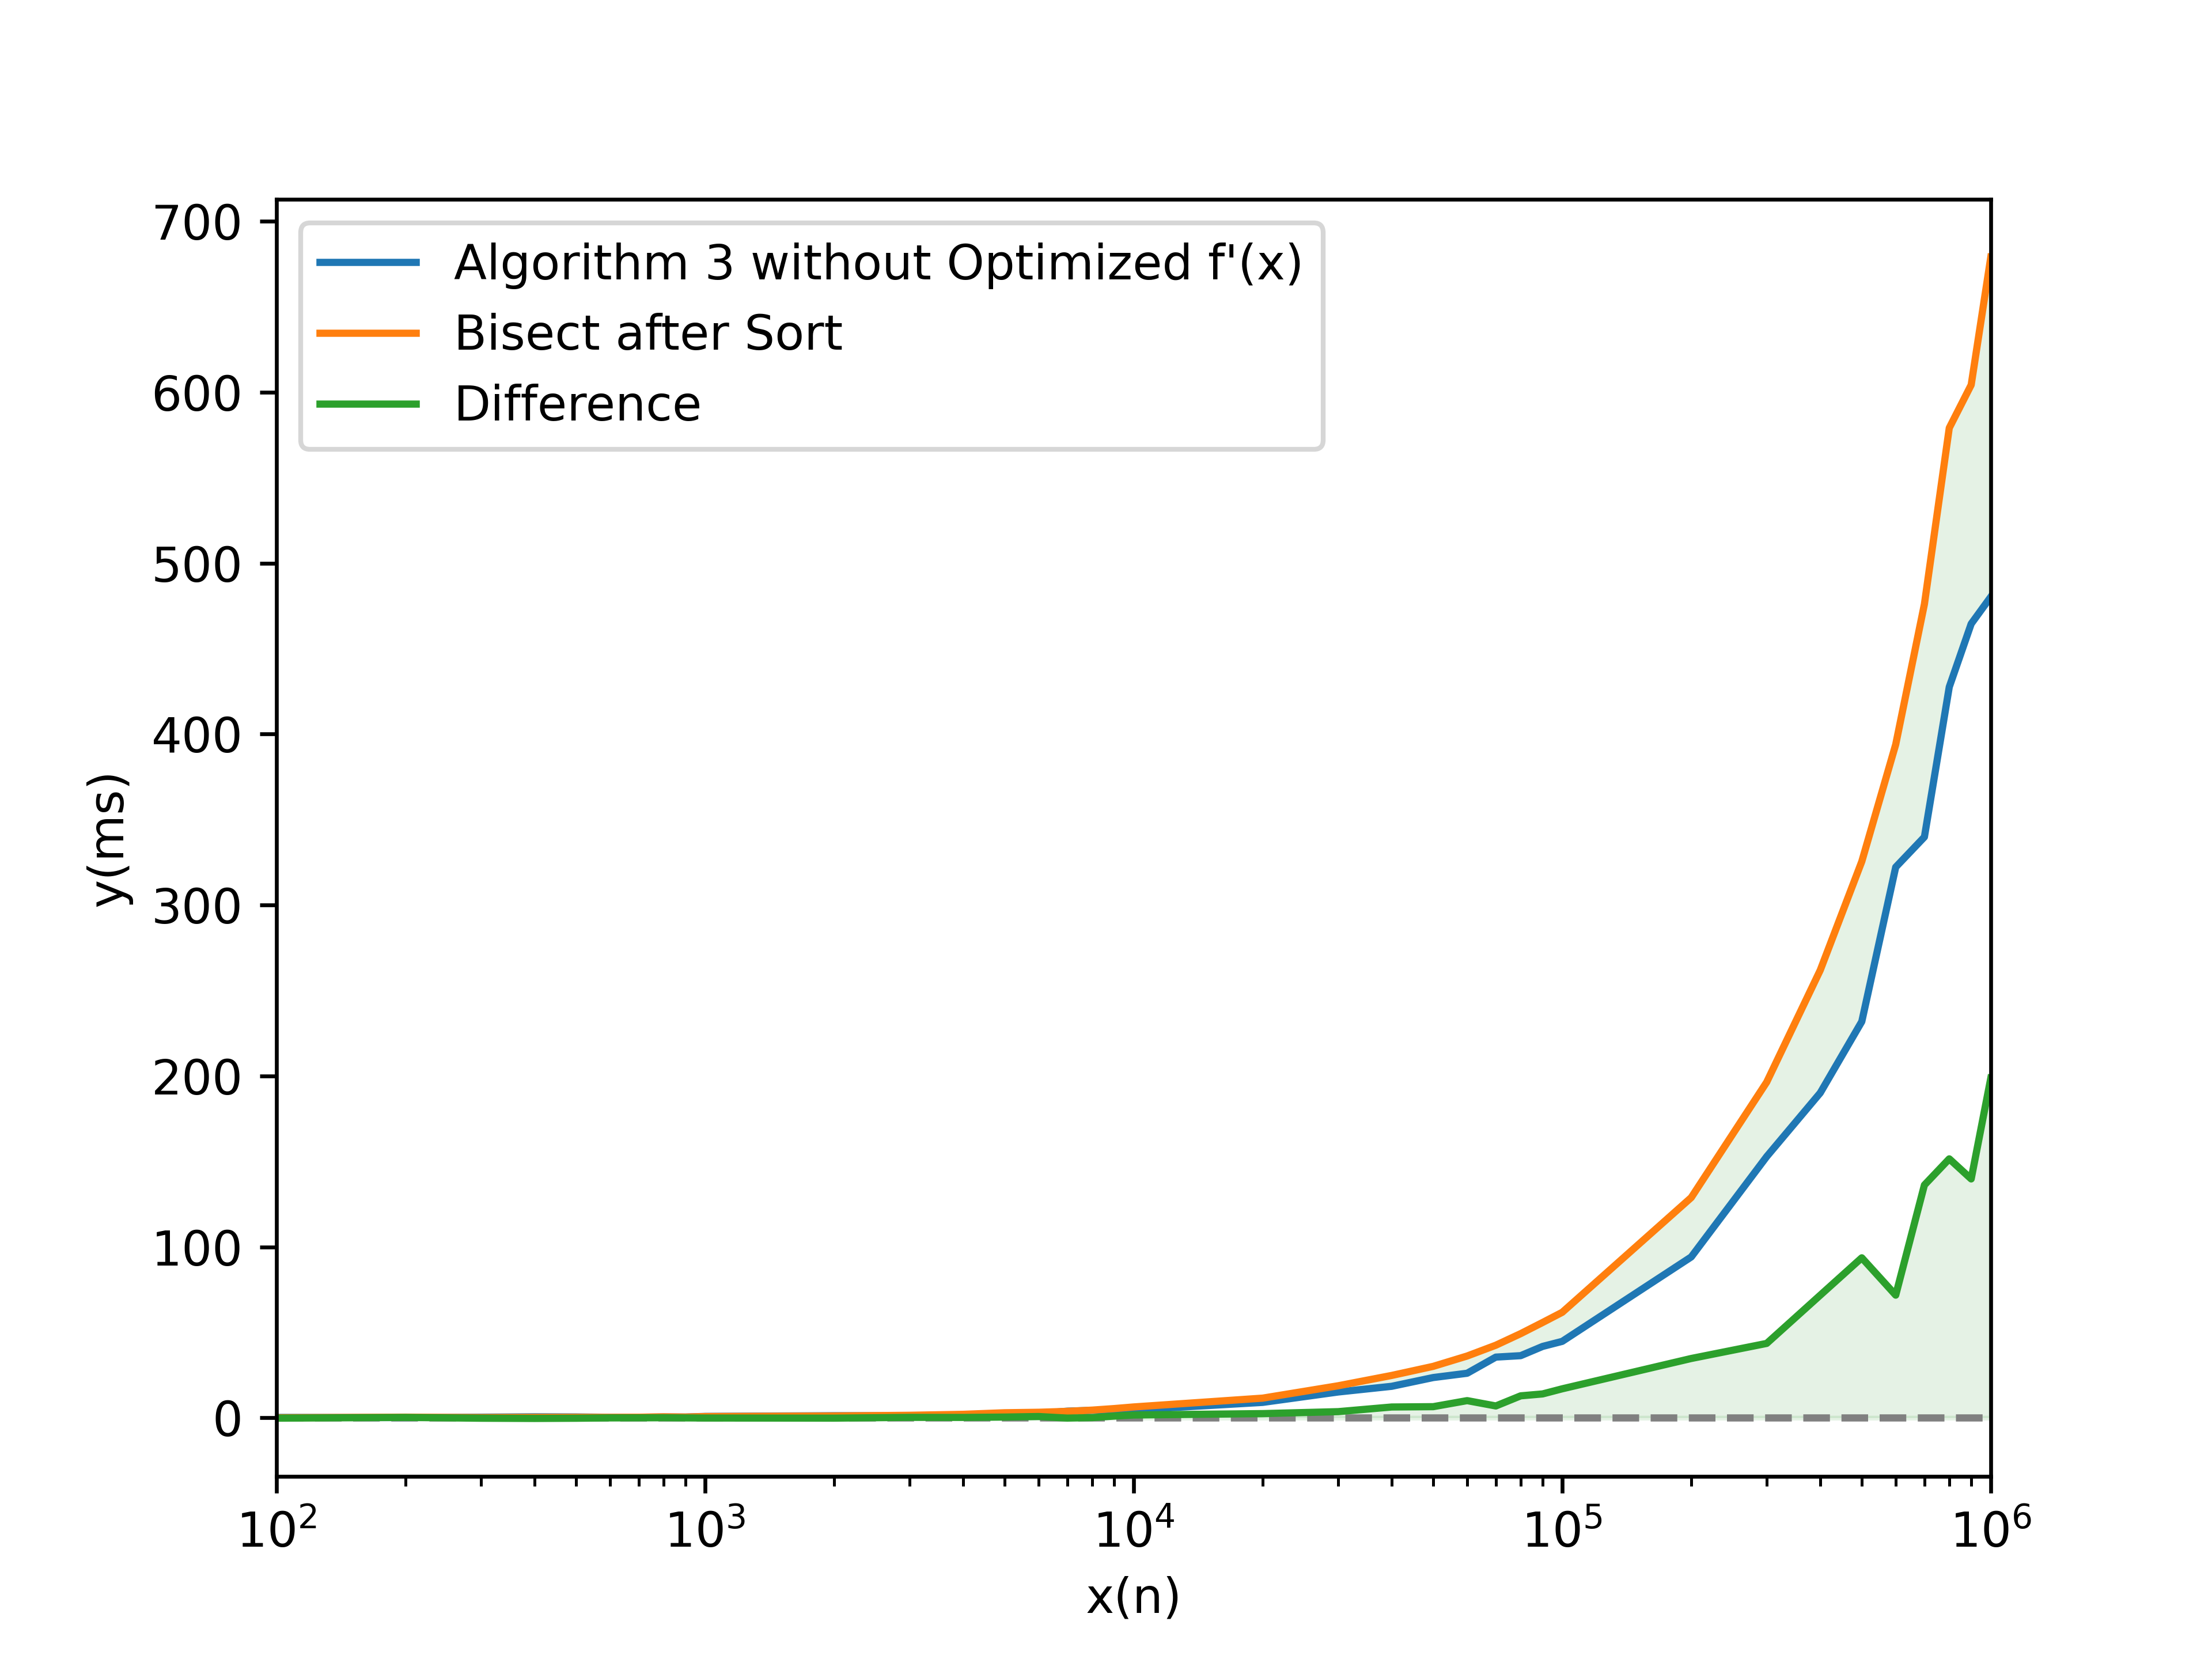
\includegraphics[width=0.5\textwidth]{figures/Compare.png}
    \caption{性能对比分析}
    \label{Compare}
\end{figure}

性能对比分析及绘图的源代码已经上传至 GitHub 仓库 \href{https://github.com/xqm32/unix-report-python}{https://github.com/xqm32/unix-report-python}。